\chapter{Short explanation of the tools}\label{explanation-tools}
Before we compare the tools, a brief explanation. When were they found? What are they focused on? Where do they excel? 

\section{Adobe XD}
Adobe XD is a user experience software manufactured by Adobe. Until 2010 Adobe Photoshop was considered the go-to design tool for both user experience and user interfaces. This completely changed with the release of Sketch, see \autoref{explanation-tools-sketch}. Adobe could not immediately respond but after a series of beta releases, Adobe released Adobe XD (Experience Design) in October 2017. 

The numbers of users is increasing rapidly. Adobe does its utmost to release new features as fast as possible. It is compatible with both Windows and macOS, allowing files to be easily exchanged between the operating systems, countering Sketch's macOS only software.

\section{Figma}
Figma is a cloud-based user experience software released in May 2016. It runs completely in the browser and therefore works on any operating system: macOS, Windows, Linux... 

It was presumed that the web application would lack in performance. To date, Figma is able to match Sketch's native performance and can even outshine it in some cases . Jamie Wong, a developer at Figma, wrote an article about performance: \url{https://www.figma.com/blog/figma-faster}

Figma has also attached a lot of importance to team collaboration. They are convinced that collaboration makes or breaks a tool. Several people should be able to view and edit files simultaneously.

\section{Invision Studio}\label{sec:invision-explanation}
Invision Studio is a very new user experience software released in the beginning of 2019. With its software it has mainly focused on allowing designers to build very advanced animations and interactions. This is beautifully displayed in a promotional video found at the top of the following page, \url{https://www.invisionapp.com/studio}.

Studio is just one of Invision's applications. The company tries to encompass the entire design flow. Below are the other software they offer:

\begin{itemize}
    \setlength\itemsep{-0.5em}    
    \item{Invision Inspect, an application specifically designed for developers. As a developer you don't want to spend hours switching between prototypes and your design to make things look right. Invision Inspect will automatically translate prototypes into detailed specs.}
    \item{Invision Craft, a plugin for Sketch and Photoshop to automate tedious actions }
    \item{Invision Freehand, an infinite whiteboard to rapidly capture feedback and work out ideas collaboratively without spending time to make it presentable}
    \item{InVision DSM, short for Design System Manager, is a platform specifically created for team collaboration. It brings developers, designers and stakeholders into a unified workflow.
    }
\end{itemize}

\section{Framer}
Two product designers at Facebook, K. Bok and J. Van Dijk, often found themselves pitching new application ideas. At the time, the prototypes they presented were static. They contained no interaction, no animations. Both of them felt frustrated with the few possibilities they had to create interactive prototypes.

Originally, they created Framer.js, a Javascript framework, to create interactive prototypes using code. The framework became very popular. They decided to create a macOS application that brings together the framework with a visual editor. That way you can immediately see the results, but you can also change visual aspects with ease.

This expanded to a tool called Framer X. Which to this day is still actively in development, but limited to macOS. With the rise of Figma, a web-based prototyping tool. Framer took notes and released Framer on web. Framer on web is still very new. It released the 28th of May, a week before this is written. They are slowly moving away from the coding experience and are adding more design capabilities, comparable to those from Figma.

\section{Axure RP}
Axure RP, short for rapid prototyping, is one of the first advanced prototyping tools ever created. In fact this year the software tool celebrates its 15th anniversary. 

When it comes to prototyping Axure has taken a very different approach compared to its competitors. Software like Sketch and Adobe XD put visual design first, until lately prototyping was additional. Axure on the other hand is specifically build for functional prototyping and interactions.

Although visual design can be done in Axure, it is also possible to import design files from Adobe XD, Sketch and Figma.

However the learning curve of Axure is quiet steep. For instance, in \autoref{fig:axure-interaction-example}, you can see a screen capture of Axure's interactions panel. It contains an if-statement that triggers when the page loads. 
\begin{figure}[H]
\centering
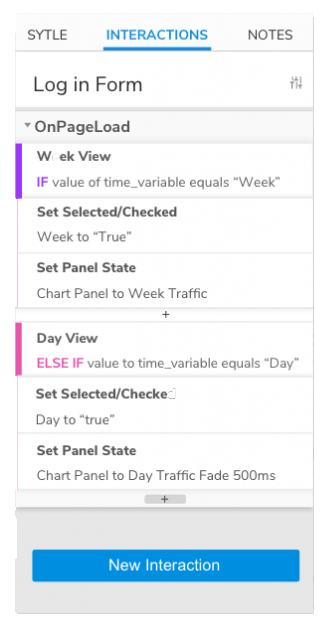
\includegraphics[scale=.5]{figures/axure-rp/interaction-example.png}
\caption{Axure interaction.}
\label{fig:axure-interaction-example}
\end{figure}

\section{Sketch}\label{explanation-tools-sketch}
Sketch is user experience software developed by the Dutch company Bohemian Coding. It was first released in September 2010. When Sketch first came out it completely disrupted the world of user experience. It had new prototyping concepts and collaboration functionalities that no other tool had. In 2012 they received an Apple Design Award for their very appealing design, which they were able to maintain up to this day.

Compared to the other tools Sketch is very mature and has age on his side. Although Sketch is only for macOS it has a large community and a well maintained third party plugin market. To this day it is still considered the industries favourite.
